\documentclass[conference]{IEEEtran}
\usepackage{amsmath}
\usepackage{booktabs}
\usepackage{graphicx}
\usepackage{hyperref}
\graphicspath{{../results/}}

\title{Containing Epidemics on the Global Air-Transport Network:\\
Budget, Centrality, and the Epidemic Threshold}

\author{
\IEEEauthorblockN{Krish Dhola (202301189), Prince Sojitra (202301126), Jenish Vasani (202301057)}
\IEEEauthorblockA{Group 22}
}

\begin{document}
\maketitle

\begin{abstract}
We study how limited airport closures affect epidemic spreading on a network derived from global air-transport routes. The analysis combines centrality-based intervention strategies, Euler-integrated SIR dynamics, and network resilience measurements. Airports are ranked using degree, closeness, betweenness, and eigenvector centrality, and the resulting strategies are compared with random closure under equal budgets.
\end{abstract}

\section{Motivation / Problem Statement}
Air travel connects distant populations and can accelerate geographic epidemic spread. Since closing all airports is impractical, this work asks which airports should be closed under a limited budget.~\cite{keeling2005,pastorsatorras2015}

\section{Methodology}
\subsection{Network construction}
We use the OpenFlights airport and route files downloaded on 27 October 2026~\cite{openflights}. Airports are nodes and routes are undirected edges. Invalid numeric identifiers, self-loops, duplicate routes, and isolated airports are removed. The cleaned graph has 3,214 airports and 18,858 connections in seven components; its largest component has 3,188 airports and 18,833 connections. Table~\ref{tab:network} summarizes the graph used for the epidemic experiments.

\begin{table}[t]
\caption{OpenFlights network summary}
\label{tab:network}
\centering
\begin{tabular}{lr}
\toprule
Measure & Value\\
\midrule
Airports (full graph) & 3,214\\
Routes (full graph) & 18,858\\
Largest-component airports & 3,188\\
Largest-component routes & 18,833\\
Average degree (largest component) & 11.81\\
Connected components & 7\\
\bottomrule
\end{tabular}
\end{table}

\subsection{Centrality and interventions}
We calculate degree, closeness, betweenness, and eigenvector centrality using NetworkX, NumPy, pandas, and Matplotlib~\cite{networkx,numpy,pandas,matplotlib}. For a budget $b$, the top $\lceil b|V|\rceil$ airports are removed for a centrality strategy. Random closure samples the same number of airports using a fixed seed. Table~\ref{tab:centrality} lists the top airports identified by each centrality measure.

\begin{table}[t]
\caption{Top airports by centrality in the largest component}
\label{tab:centrality}
\centering
\begin{tabular}{ll}
\toprule
Measure & Top three airports (OpenFlights ID)\\
\midrule
Degree & Schiphol (580), Frankfurt (340), Charles de Gaulle (1382)\\
Closeness & Frankfurt (340), Charles de Gaulle (1382), Heathrow (507)\\
Betweenness & Charles de Gaulle (1382), LAX (3484), Anchorage (3774)\\
Eigenvector & Schiphol (580), Frankfurt (340), Charles de Gaulle (1382)\\
\bottomrule
\end{tabular}
\end{table}

\subsection{SIR threshold}
The normalized mean-field model is
\begin{equation}
\dot S=-\beta SI,\quad \dot I=\beta SI-\gamma I,\quad \dot R=\gamma I.
\end{equation}
The threshold is $R_0=\beta S_0/\gamma$. The disease-free equilibrium is stable below $R_0=1$ and loses stability at the transcritical threshold.

\begin{figure}[t]
\centering
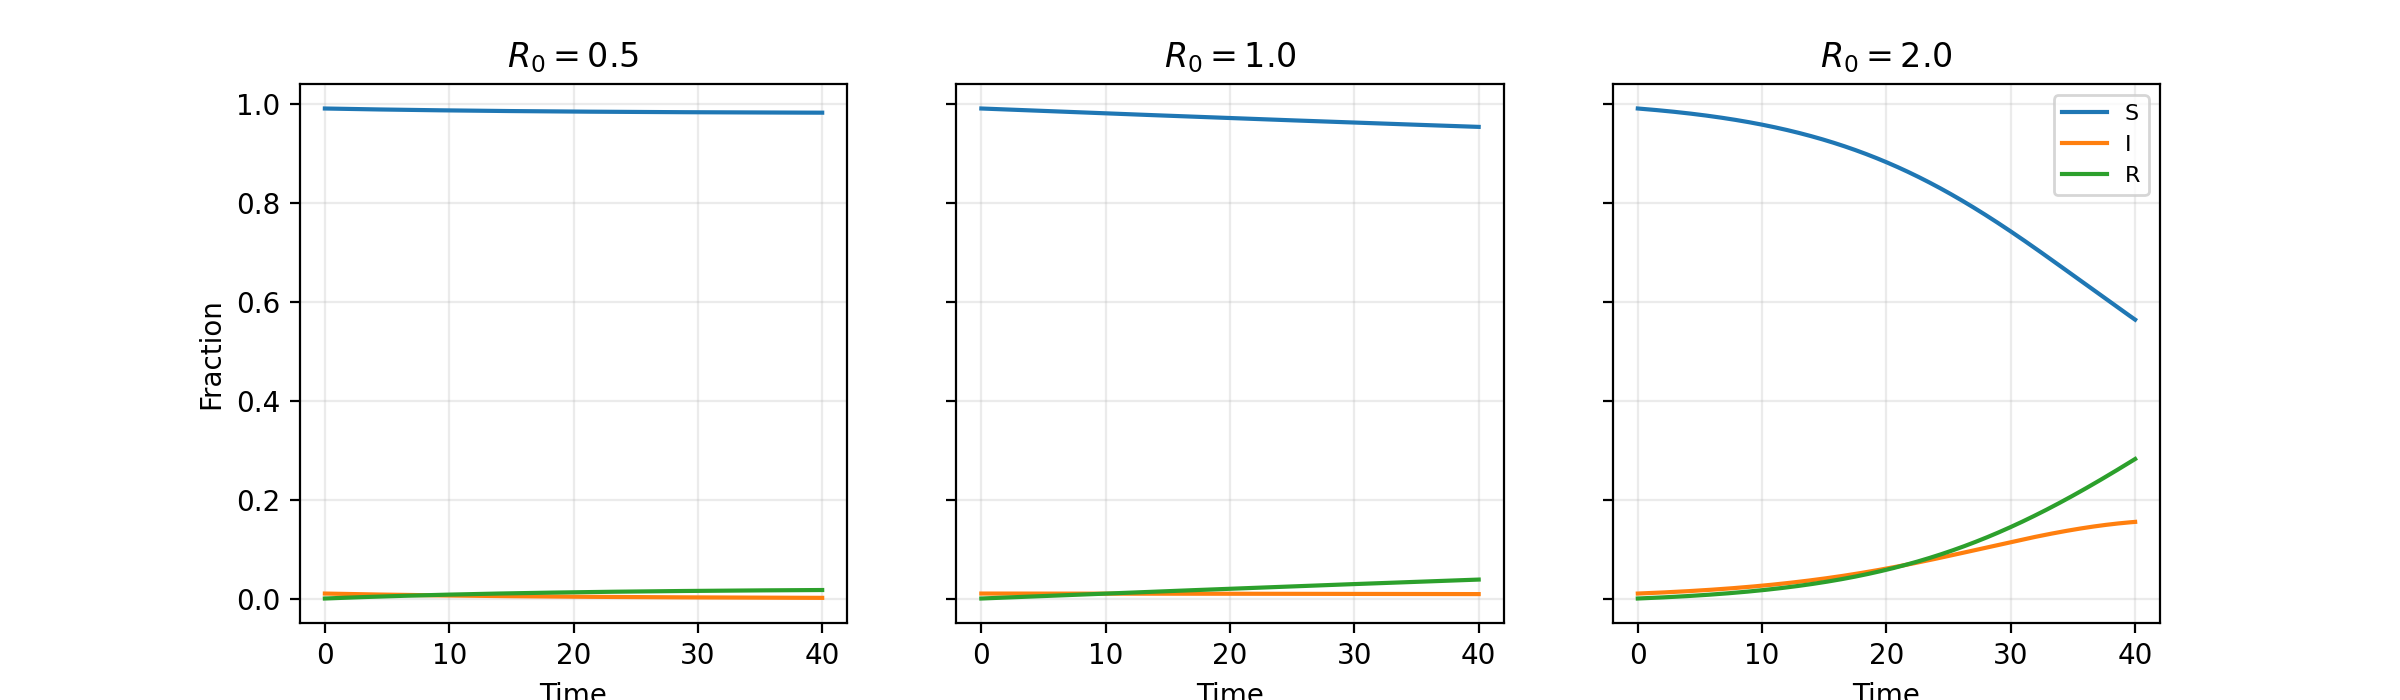
\includegraphics[width=\columnwidth]{mean_field_threshold.png}
\caption{Mean-field SIR behavior below, at, and above the epidemic threshold.}
\label{fig:threshold}
\end{figure}

\subsection{Network metapopulation model}
Each airport has susceptible, infected, and recovered populations. Local transmission is $\beta S_iI_i/N_i$, recovery is $\gamma I_i$, and an undirected graph-diffusion term couples neighbouring airports. For each compartment $X_i\in\{S_i,I_i,R_i\}$, mobility adds $\mu\left(\sum_{j\in N(i)}X_j-k_iX_i\right)$, where $k_i$ is airport $i$'s degree. Euler integration is used with $\beta=0.30$, $\gamma=0.10$, mobility rate $0.02$, normalized population one per airport, $dt=0.1$, and duration 80. The initial infected fraction is 1\% at one fixed high-degree seed airport. The seed airport is protected from closure so that every strategy is evaluated from the same initial condition. For immediate closure, selected airports and their incident routes are removed before simulation. For delayed closure, incident mobility edges are removed and local infection at closed airports is set to zero at the intervention time; their existing populations remain and can recover.

\subsection{Interventions and measurements}
We compare random, degree, closeness, betweenness, and eigenvector closures for budgets from 1\% to 20\%. Outcomes include final outbreak size, peak infection, time to peak, and largest connected component. Final outbreak size is the cumulative recovered fraction at the end of the simulation. We define containment as final outbreak size at most 5\%. The complete sweep evaluates every integer budget from 1\% to 20\%; random closure uses five independent trials.

\section{Results and Key Findings}
Figure~\ref{fig:budget} shows the complete generated real-network comparison. At a 20\% budget, closeness has the smallest final outbreak size (1.80\%), followed by degree (3.00\%), eigenvector (6.43\%), betweenness (10.11\%), and random closure (61.63\%). Degree reaches the 5\% containment criterion first, at 18%; closeness reaches it at 20%, while betweenness, eigenvector, and random closure do not reach it within the tested range. Targeted strategies reduce outbreaks more strongly, but they also fragment the network more severely. Table~\ref{tab:strategies} summarizes the final outbreak, peak infection, and connectivity outcomes at the 20\% budget.

\begin{figure}[t]
\centering
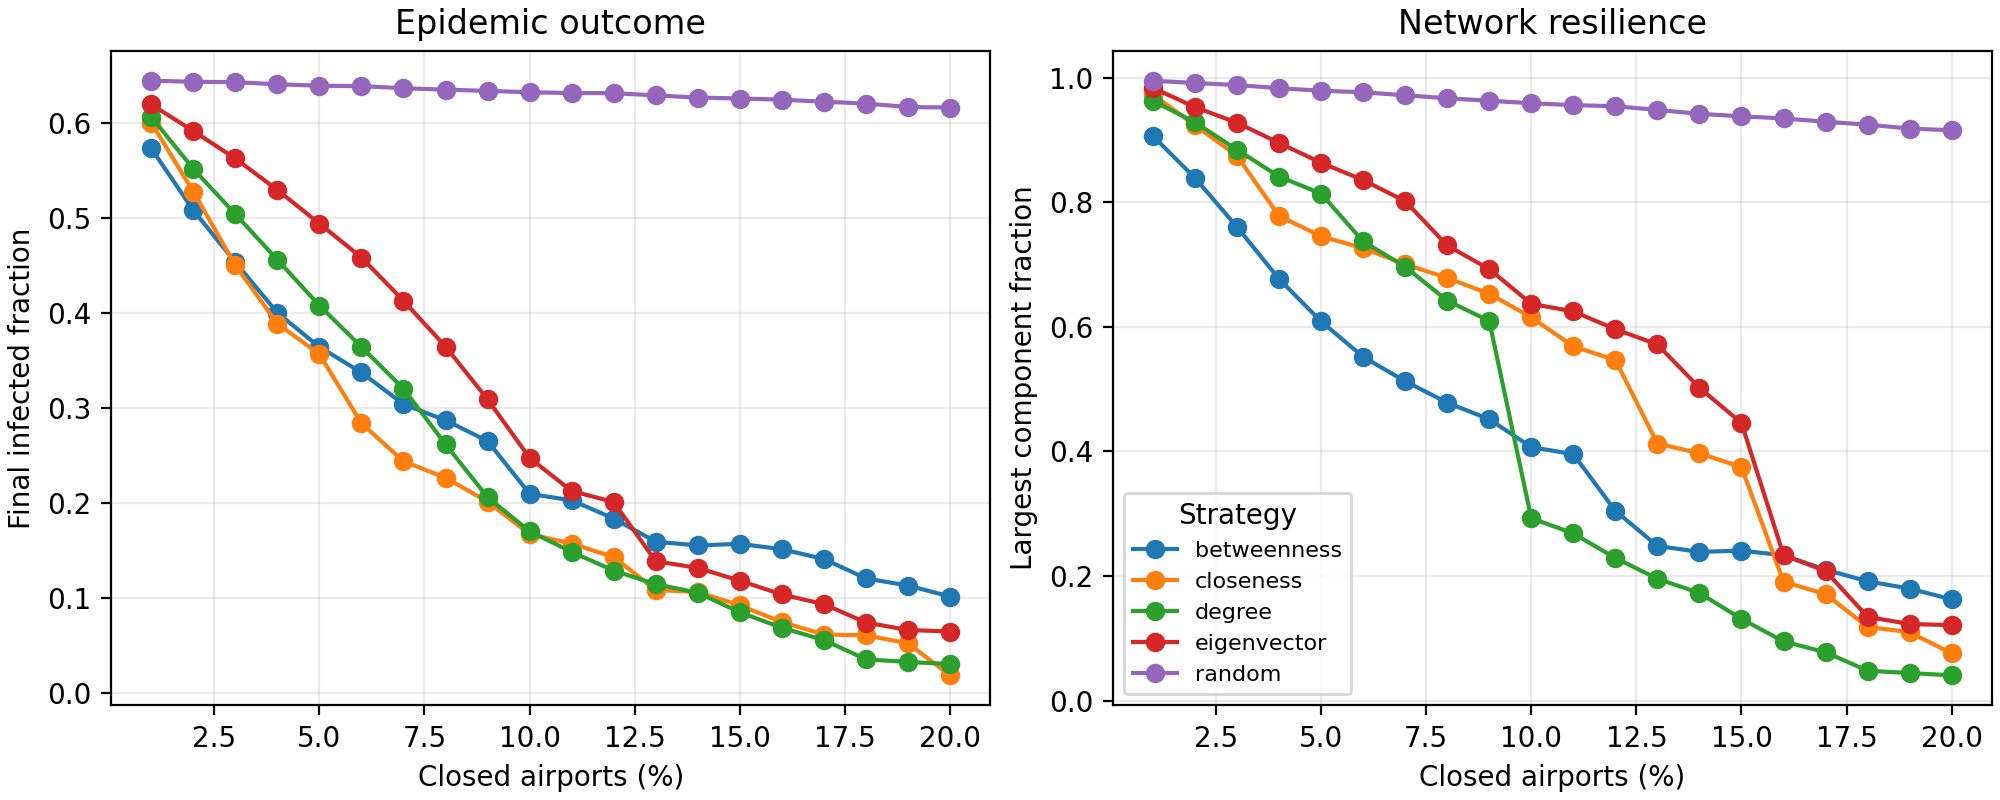
\includegraphics[width=\columnwidth]{openflights_closure_results_full.png}
\caption{Complete 1--20\% closure-budget results on the largest OpenFlights component.}
\label{fig:budget}
\end{figure}

\begin{table}[t]
\caption{Final outbreak and connectivity at a 20\% budget}
\label{tab:strategies}
\centering
\begin{tabular}{lrrr}
\toprule
Strategy & Final outbreak & Peak infected & LCC fraction\\
\midrule
Random & 61.63\% & 25.45\% & 91.55\%\\
Degree & 3.00\% & 0.80\% & 4.04\%\\
Closeness & 1.80\% & 0.59\% & 7.57\%\\
Betweenness & 10.11\% & 3.22\% & 16.24\%\\
Eigenvector & 6.43\% & 2.22\% & 12.12\%\\
\bottomrule
\end{tabular}
\end{table}

The compact synthetic comparison was used as a short-horizon implementation check across ER, BA, and WS networks at a 10\% closure budget. Because these validation runs ended at time 20 while infection was still active, they are not used for the main containment conclusion. The degree-preserving null comparison retained almost the same random-closure connectivity as the real network (96.5\% versus 96.6% largest-component fraction at 10\%), while degree-based removal produced 29.3\% for the real graph and 61.5\% for the randomized graph. This indicates that detailed topology, not only the degree sequence, affects fragmentation.

Delayed intervention was evaluated with a fixed 10\% betweenness closure budget. With immediate, 20-unit, and 40-unit intervention, final outbreak sizes were 18.83\%, 54.15\%, and 57.02\%, respectively, and peak infected fractions were 6.30\%, 23.21\%, and 24.44\%. Thus, intervening later substantially increases outbreak size in this model.

\section{Discussion / Analysis}
The real network is heterogeneous: a small set of airports has a large role in connecting otherwise weakly connected regions. Degree and closeness performed best for reducing the cumulative outbreak under the tested parameters, whereas betweenness caused strong fragmentation but did not achieve the 5\% containment criterion by 20\%. This demonstrates that structural importance for connectivity and epidemic suppression need not be identical. The appropriate strategy depends on whether the objective prioritizes epidemic reduction, connectivity preservation, or a weighted combination of both.

The model has several limitations. OpenFlights route records do not provide passenger populations or time-varying traffic, so normalized airport populations and unweighted routes are used. The SIR parameters are scenario parameters rather than estimates for a particular disease. Finally, the intervention comparison measures structural removal and does not model rerouting or behavioral adaptation.

\section{Conclusion}
This project provides a reproducible framework for comparing airport closure strategies on a real flight network. The mean-field model validates the epidemic threshold, while the metapopulation model connects local SIR dynamics to global network structure. The final parameter sweep identifies the smallest budget satisfying the stated containment criterion and quantifies its connectivity cost.

\bibliographystyle{IEEEtran}
\bibliography{references}
\end{document}
